
\myChapter{Ulteriori applicazioni e conclusioni}
In quest'ultimo capitolo elencheremo ulteriori possibili campi di applicazione dei GA, ricongiugendoci con quanto visto nella risoluzione del problema del cammino minimo, per poi rimanere, successivamente, nell'ambito di casi di studio relativi ai grafi, terminando con una visione generale sugli sviluppi attuali e futuri dei GA, consci di quanto osservato durante la tesi.
%\section{Ulteriori applicazioni sui grafi}

Sebbene il precedente capitolo vertesse solamente sull'implemetanzione, non ottimale, di un GA nella risoluzione del problema del cammino minimo, durante il tirocinio sono stati presi in considerazione molteplici casi di studio riguardo ai grafi; in particolare la nostra attenzione si \`e soffermata principalmente su due problemi molto conosciuti nel mondo scientifico: il problema del commesso viaggiatore \cite{tsp1} (Travelling Salesman Problem, TSP, di cui parleremo molto rapidamente) e della colorazione di un grafo\cite{graphcol6}.
\section{Il problema del commesso viaggiatore}
Per chi \`e esperto del settore questo problema sar\`a ben noto, ma comunque descriveremo velocemente in cosa consiste citando la domanda che esso pone:
\vspace{3mm}

\textit{Data una lista di citt\`a e date le distanze fra coppie di esse, qual \`e il cammino minimo possibile che attraversa tutte le citt\`a e che termina in quella di partenza?}
\vspace{3mm}
\begin{figure}[H]%
    \centering
    %\hfill
    \subfloat[Insieme di citt\`a]{{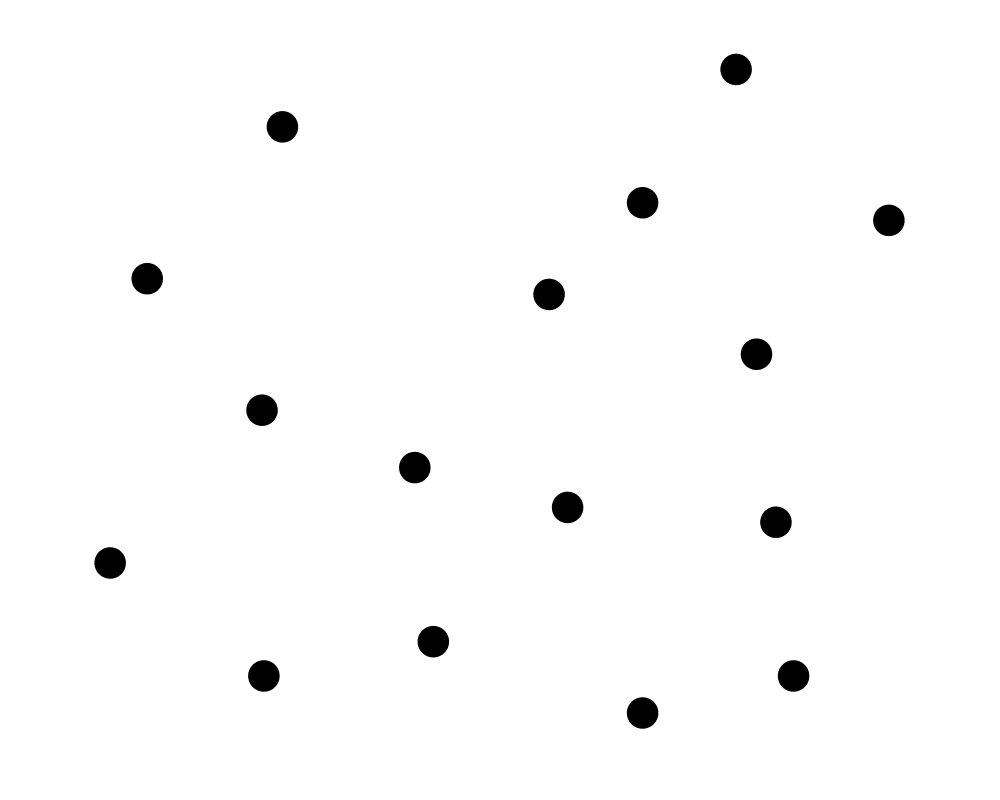
\includegraphics[width=0.5\linewidth]{Images/tspStart.png}}}%
    %\qquad
    %\hfill
    \subfloat[Una possibile soluzione]{{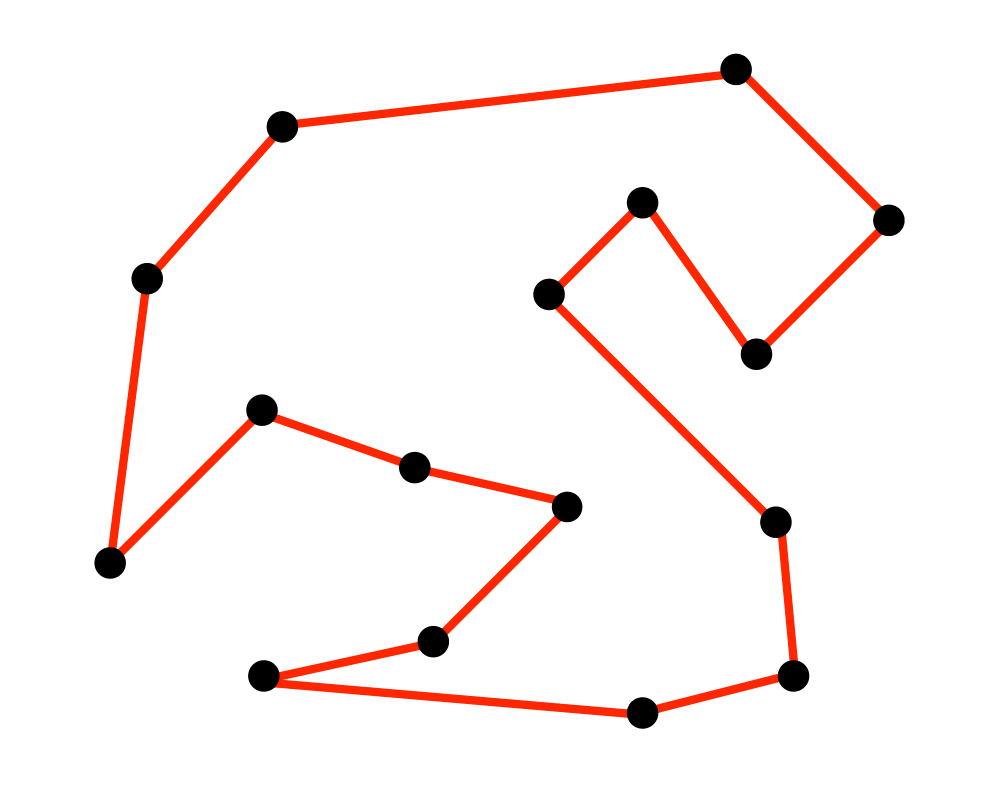
\includegraphics[width=0.5\linewidth]{Images/tspEnd.png}}}%
    %\hfill
    %\caption{Confronto fra la prima e l'ultima generazione per la nuova funzione considerata}%
    \caption{Il problema del commesso viaggiatore, fonte: algorist.com}
    \label{fig:tsp}%
\end{figure}
A prima vista la domanda posta dal problema potrebbe risultare simile a quella vista all'inizio del capitolo 5, la differenza consiste nel fatto che essa richieda il calcolo del migliore \textit{ciclo hamiltoniano} che un possibile commesso possa intraprendere fra tutte le citt\`a.

La maggiore difficolt\`a risiede, per determinare l'efficacia di un possibile GA, nel fatto che mancano algoritmi efficienti per la risoluzione nel caso di un'ingente quantit\`a di citt\`a, lasciandoci senza valori di riferimento come lo era stato l'algoritmo di Dijkstra nel capitolo precedente; il problema, che viene usato anche come standard di valutazione per numerosi algoritmi di ricerca, \`e di una complessit\`a computazionale elevata (pari ad O(n!) per algoritmi esatti, con n numero di citt\`a e considerato il caso peggiore in cui ogni nodo risulta connesso a tutti gli altri), di fatto \`e stato possibile risolvere il problema con precisione fino ad una decina di migliaia di citt\`a, ottenendo non grandi margini di errori per un'insieme di milioni di citt\`a.
\vspace{3mm}

Come per la ricerca del cammino minimo, anche il TSP, a sua volta in maniera simile, pu\`o essere espresso come un problema basato sui grafi: le citt\`a corrisponderebbero ai vertici, le congiunzioni fra le citt\`a risultano gli archi e le distanze come i pesi di tali archi; il tutto, dunque, si trasforma in un problema di minimizzazione che parte e termina in uno stesso vertice, effettuando la visita una ed una sola volta di ogni altro vertice in un grafo non orientato e pesato.
\vspace{3mm}

Seppur paradossale, l'approccio con i GA risulta, secondo \cite{path4}, di pi\`u semplice implementazione rispetto al calcolo del cammino minimo: i cromosomi rappresentanti i vari cicli, avrebbero tutti la stessa lunghezza e sappiamo come la gestione di lunghezze differenti causi maggiore complessit\`a in fase di implementazione (abbiamo avuto la possibilit\`a di sperimentare sulla nostra pelle questo fatto).
\vspace{3mm}

I tentativi di dare una soluzione al problema tramite l'uso dei GA sono stati molti, in particolare Heinrich Braun \cite{tsp2} \`e stato in grado (migliorando quanto fatto da Muhlenbein e colleghi \cite{tsp3}) di trovare una soluzione ottimale fino a 442 citt\`a; inoltre sono stati effettuati diversi studi su quanto le scelte di implementazione effettuate sui vari operatori \cite{tsp5} (che ricordiamo per l'ennesima volta essere: selezione, crossover e mutazione) influiscono sull'efficacia nel trovare il ciclo minimo, in particolare una buona scelta fra le possibili varianti della selezione permette, come dimostrato da \cite{tsp4}, di ottenere risultati migliori.
\vspace{3mm}

Avendo trattato fino ad ora due dei maggiori problemi di minimizzazione incentrati su cammini e cicli minimi, passeremo nella prossima sezione ad osservare un altro ambito di applicazione dei GA sempre relativo ad un problema riguardante i grafi.
%Inoltre, sempre riguardo gli operatori nel contesto del TSP, 
%\begin{center}
%\begin{table}[]
    %\centering
%    \begin{tabular}{C|C|C|C|C}
    %     &  \\
     %    & 
 %   \end{tabular}
%    \caption{Caption}
%    \label{tab:my_label}
%\end{table}
%\end{center}
\section{Colorazione di un grafo}
La colorazione di un grafo consiste, come il nome ci suggerisce, nell'assegnare ad ogni vertice di un grafo un colore (od etichetta) in modo tale che nessun vertice condivida la stessa etichetta con quelli a lui adiacenti, pi\`u nel dettaglio il problema pu\`o essere espresso come:
\vspace{3mm}

\textit{Dato un grafo G, calcolare il \textit{numero cromatico} $\chi(G)$, ovvero trovare il numero minimo di colori necessari affinch\'e nessun nodo condivida un colore con quelli a s\'e adiacenti.}
\vspace{3mm}

Casi analoghi riguardano la colorazione delle facce di un grafo planare o degli archi, ma in questa sezione discuteremo solamente della colorazione dei vertici e della nostra semplice implementazione in Java.
\vspace{3mm}
\begin{figure}[H]
    \centering
    \hfill
    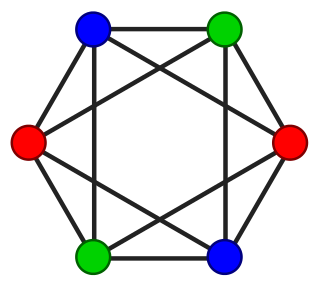
\includegraphics[width=0.5\textwidth]{Images/graphColoring.png}
    \hspace*{\fill}
    \caption{Colorazione di un grafo}
    \label{fig:graphColoring}
\end{figure}
L'idea per realizzare il GA \`e sicuramente pi\`u agevole di quanto abbiamo fatto nel capitolo precedente, ma in certi versi simile: gli operatori fondamentali sono sempre quelli (potremmo agire sulla selezione ed usarne una diversa da quella a torneo, oppure cambiando il crossover), per\`o ci sarebbe il vantaggio di poter usare codifiche di dimensione costante pari al numero di vertici; i cromosomi nascenti da esse avrebbero i geni rappresentanti i colori (o meglio un intero/stringa che identifica univocamente il colore).
\begin{figure}[H]
    \centering
    \hfill
    
\includegraphics[width=0.95\textwidth]{Images/coloring.png}
    \hspace*{\fill}
    \caption{Codifica di un possibile individuo, ad ogni intero corrisponde un colore}
    \label{fig:coloring}
\end{figure}
Viene naturale pensare alla funzione di fitness come alla somma, per ogni cromosoma, dei vertici adiacenti aventi lo stesso colore assegnato; di conseguenza i migliori cromosomi hanno valori di fitness minori rispetto agli altri, per tale ragione l'implementazione ed il ragionamento da eseguire combacia quasi perfettamente con quanto visto per la ricerca del cammino minimo.
\vspace{3mm}

%\textbf{da inserire: codice delle funzioni cardine e commenti}
%
Abbiamo implementato anche noi stessi un algoritmo volto alla colorazione dei grafi, ponendo le fondamenta su quanto fatto da \cite{graphcol1}, ovvero usando il GA fino ad un arbitrario numero di iterazioni per poi concludere con un algoritmo ad hoc (\textit{wisdom of artificial crowds}) in modo da ridurre il margine di errore. Il codice risulta avere la stessa strutture di quanto implementato nel capitolo 4, di fatto non riporteremo il sorgente in appendice, ma spenderemo comunque qualche parola sulle nostre scelte implementative.
\vspace{3mm}

La creazione della prima generazione, a differenza per il problema del cammino minimo, \`e completamente casuale: questo ci permette di avere una popolazione pi\`u ampia e, di conseguenza, maggiori probabilit\`a di raggiungere il risultato ottimale. Dato che i cromosomi hanno dimensione fissa (pari al numero di nodi del grafo), non dobbiamo eseguire controlli ulteriori nell'operatore di selezione e nella mutazione (cosa che ci ha creato non pochi problemi nella ricerca del cammino minimo).
\vspace{3mm}

Gli operatori di selezione, crossover e mutazione rimangono pressoch\'e invariati rispetto a quanto osservato nel capitolo passato; la selezione ed il crossover rimangono, rispettivamente, nella loro variante a torneo ed a punto singolo (senza il bisogno di eliminare nodi duplicati), mentre la mutazione viene enormemente semplificata: scelto casualmente un gene con probabilit\`a \textit{pMutation}, tale operatore non fa altro che impostare il valore del gene ad uno degli altri colori possibili, rendendolo estremamente pi\`u veloce di quanto fatto nel capitolo 4.
\vspace{3mm}

Non ci resta, dunque, che introdurre una possibile funzione di fitness, la quale \`e stata gi\`a in parte descritta in un paragrafo precedente: abbiamo deciso che la funzione sia data dalla somma fra il numero di archi che connettono vertici aventi lo stesso colore assegnato (l'operazione prevede lo scorrimento del cromosoma e l'uso di una matrice di adiacenza) ed il numero di colori usati dal cromosoma.
\vspace{3mm}

\begin{Large}
{$$f(x)=\sum_{i=0}^{|V|-2}(\sum_{j=i+1}^{|V|-1}k)+\#used\_colors$$ }
\end{Large}
con k=$\begin{cases}
$1$, & \text{se v[i] e v[j] sono adiacenti e hanno lo stesso colore} \\
$0$, & \text{altrimenti}
\end{cases}$
\vspace{3mm}

Quest'ultimo parametro (\textit{\#used\_colors}) \`e indispensabile altrimenti i cromosomi usanti tutti colori differenti per la colorazione dei nodi risulterebbero decisamente migliori, pur essendo lontani dall'esserlo. La seguente immagine mostra un chiaro esempio in cui questo parametro risulta essere fondamentale.
\begin{figure}[H]%
    \centering
    %\hfill
    \subfloat[Esempio senza collisioni]{{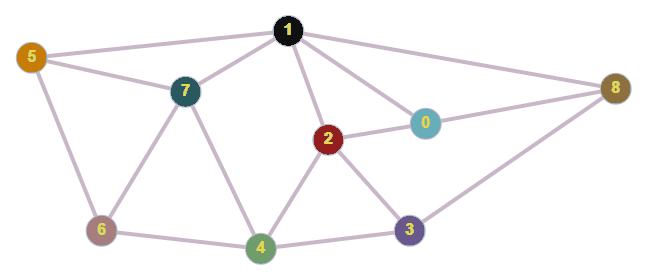
\includegraphics[width=0.5\linewidth]{Images/coloring2.png}}}%
    %\qquad
    %\hfill
    \subfloat[Esempio con collisioni]{{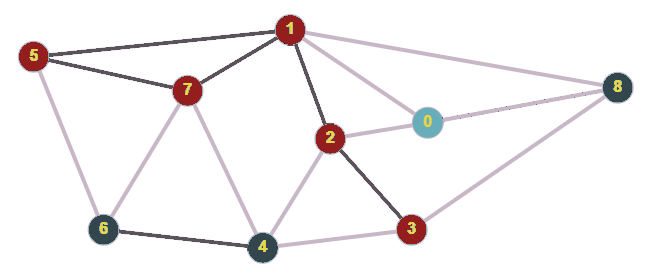
\includegraphics[width=0.5\linewidth]{Images/coloring3.png}}}%
    %\hfill
    %\caption{Confronto fra la prima e l'ultima generazione per la nuova funzione considerata}%
    %\caption{Il problema del commesso viaggiatore, fonte: algorist.com}
    \caption{Due esempi di colorazione di un grafo, il secondo risulta milgiore ai fini della ricerca con un GA}
    \label{fig:coloring2}%
\end{figure}
\vspace{3mm}
Utilizzando la funzione di fitness previamente descritta, possiamo notare come la soluzione proposta a sinistra risulti avere un valore di fitness pari a $9$ derivante solo dai colori usati, mentre la seconda pur avendo la stessa fitness utilizza solamente tre colori; se non avessimo inserito il parametro \textit{\#used\_colors} la prima colorazione sarebbe risultata la migliore in assoluto, ma non avrebbe assolutamente raggiunto $\chi(G)$ e questo avrebbe potuto indurre il nostro algoritmo su una strada sbagliata, pertanto, ai fini della ricerca, la seconda soluzione risulta la migliore per il proseguimento del GA (potremmo, a nostra scelta, eseguire il prodotto fra \textit{\#used\_colors} ed un valore fra 1 e 2, a seconda di quanto desideriamo che tale parametro influisca sul lavoro del nostro algoritmo).
\vspace{3mm}
%Per scelta nostra abbiamo usato lo stesso grafo visto nel capitolo 5 per testare il nostro algoritmo scritto in Java, seppur applicando scelte implementative diverse: la creazione della prima generazione \`e completamente casuale, inoltre vi sono due metodi differenti di mutazione e selezione (uno per quando il valore di fitness risulta molto basso, uno in ogni altro caso \cite{graphcol1}).
%\vspace{3mm}

Il nostro Ga, con le giuste modifiche, risulta avere un potenziale molto elevato dato che il problema della colorazione dei grafi trova le sue applicazioni pratiche in numerevoli campi, fra i quali:
\begin{itemize}
    \item Colorazione delle mappe \cite{graphcol3}.
    \item Scheduling dei processi \cite{graphcol8}.
    \item Allocazione dei registri \cite{graphcol7}.
    \item Ai giochi, caso pi\`u noto \`e sicuramente il sudoku \cite{graphcol2} \cite{graphcol5},
    %di cui daremo una rapida visione per concludere il nostro capitolo.
%\end{itemize}
%Parlando velocemente del sudoku, di cui a nostro parere personale risulta l'esempio pi\`u intuitivo di applicazione della colorazione, possiamo immaginare ogni cella del gioco come un vertice del nostro grafo, ognuno di questi vertici sono connessi a quelli presenti nello stessa quadrante e nella stessa riga/colonna.
%La seguente immagine mostra chiaramente quanti sono gli archi facenti parte del grafo rappresentante le celle del sudoku (blu quelli fra celle dello stesso quadrante, rossi per quelle sulla stessa riga e colonna).
%\vspace{3mm}
    \begin{figure}[H]%
        \centering
        %\hfill
        \subfloat[Sudoku vista 2d]{{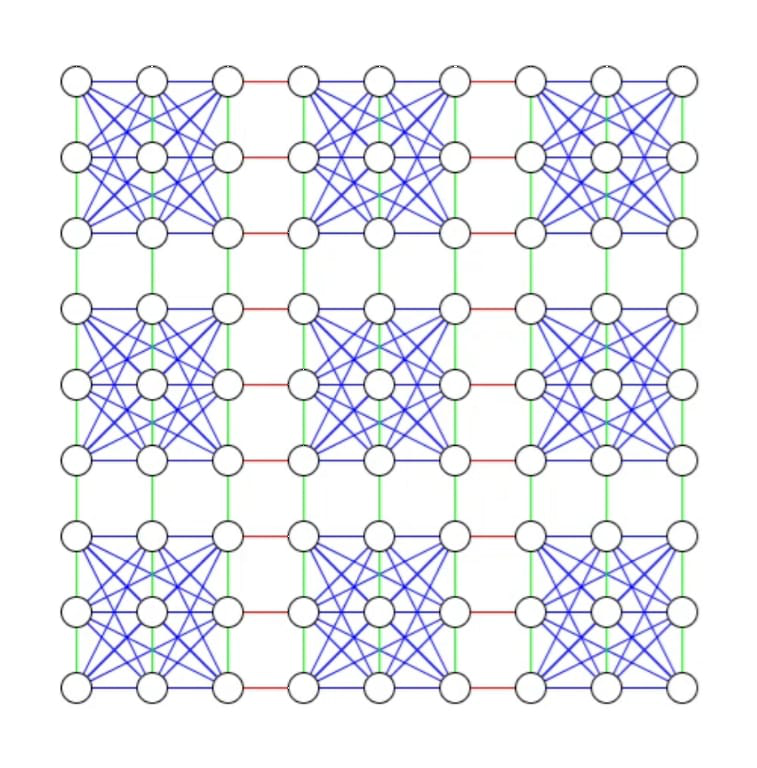
\includegraphics[width=0.5\linewidth]{Images/sudoku2d.png}}}%
        %\qquad
        %\hfill
        \subfloat[Sudoku vista 3d]{{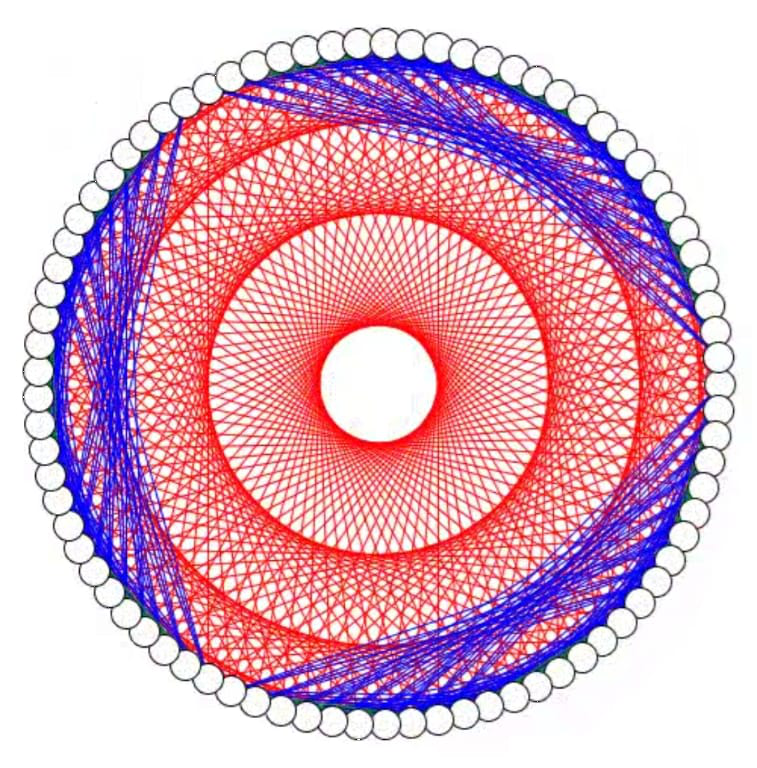
\includegraphics[width=0.5\linewidth]{Images/sudoku3d.png}}}%
        %\hfill
        %\caption{Confronto fra la prima e l'ultima generazione per la nuova funzione considerata}%
        %\caption{Il problema del commesso viaggiatore, immagine trovata dal web}
        \caption{Rappresentazione degli archi del grafo basato sul sudoku}
        \label{fig:sudoku2d3d}%
    \end{figure}
    data la sua predisposizione come strumento di analisi e confronto per gli algoritmi di ricerca.
\end{itemize}
%Considerato che ci sono $9$ quadranti (stesso vale per le righe e colonne), \`e immediato pensare al sudoku come un problema di colorazione con $9$ colori.
%\vspace{3mm}
%\begin{figure}[H]
%    \centering
%    \hfill
%    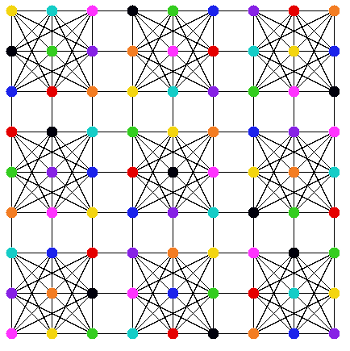
\includegraphics[width=0.50\textwidth]{Images/sudoku.png}
%    \hspace*{\fill}
%    \caption{La colorazione applicata al sudoku, opera di http://www.open-graphtheory.org/}
%    \label{fig:sudoku}
%\end{figure}
%Di fatto, sono state trovate varie soluzioni al gioco del sudoku tramite i GA: se non vogliamo rimanere nell'ambito della colorazione dei grafi, allora vale la pena citare il lavoro eseguito da Mantere e Koljonen \cite{graphcol2} ed ampliato da Deng e Li \cite{graphcol5}, i quali hanno usato un approccio differente (seppur sempre tramite l'uso dei GA) nella creazione e soluzione dei sudoku: non andando nei minimi dettagli, la maggior differenza risiede nella codifica dei cromosomi, i quali non risultano pi\`u essere composti dai colori assegnati ai vertici, ma dai valori delle celle stesse (fra i quali alcuni sono "fissi" ovvero iniziali).
%\vspace{3mm}
%La decisione di prendere in esame rapidamente il sudoku \`e scaturita dal fatto che tale gioco \`e molto noto in ambito scientifico data la sua predisposizione come strumento di test/confronto per gli algoritmi di ricerca, oltre al fatto di essere un buon esempio da suggerire in ambito accademico agli studenti per provare e capire direttamente come lavorare con un GA (abbiamo descritto velocemente due approcci, ma potrebbero sicuramente esisterne altri).
%Oltre ai due casi di esempio portati in questo capitolo, ne esistono sicuramente tantissimi altri, ma abbiamo preferito rimanere legati all'ambito dei grafi per non disorientare troppo il lettore ed appannare le loro idee, d'altronde entrambi gli esempi presenti in queste sezioni sono un piccola goccia in un vasto mare di applicazioni; di questi ne parleremo nel prossimo ed ultimo capitolo.
%La decisione di prendere come esempio rapido il sudoku \`u scaturita dal fatto che tale gioco \`e usato in ambito scientifico per
Dopo aver esposto due ulteriori ambiti di applicazioni dei GA sui grafi, dedicheremo le prossime due sezioni a concludere la tesi, esponendo rapidamente altri campi di utilizzo dei GA, per poi concludere con una piccola riflessione sul loro futuro.
\section{I GA nei vari ambiti scientifici}
Gi\`a Goldman nella sua opera maggiormente nota \cite{goldberg1} inser\`i una esaustiva lista di campi di applicazione dei GA, i diversi ambiti andavano dalla biologia all'informatica, dall'ingegneria meccanica \cite{end1} all'image processing\cite{end2} ed al riconoscimento di pattern \cite{end3}, fino ad arrivare alla finanza\cite{end6} ed alla fisica. Abbiamo sempre ribadito quanto i GA siano flessibili, il loro ampio raggio d'impiego ne \`e la testimonianza pi\`u diretta.
%\vspace{3mm}
\begin{figure}[H]%
    \centering
    %\hfill
    \subfloat[Articoli per anno]{{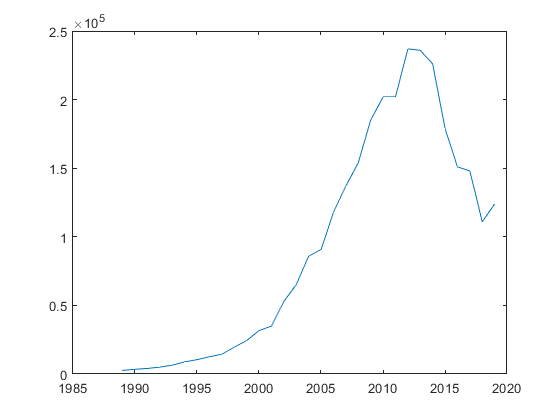
\includegraphics[width=0.5\linewidth]{Images/graph1.png}}}%
    %\qquad
    %\hfill
    \subfloat[Articoli per anno (cumulativi)]{{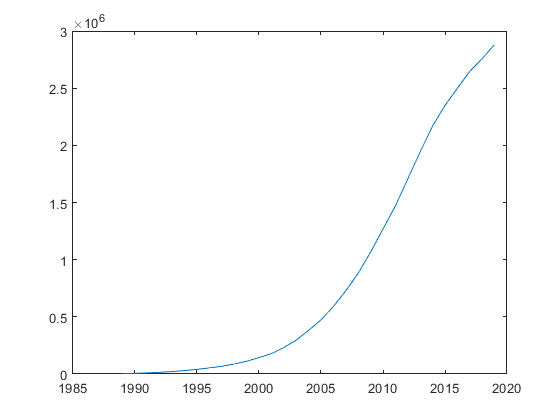
\includegraphics[width=0.5\linewidth]{Images/graph2.png}}}%
    %\hfill
    %\caption{Il problema del commesso viaggiatore, immagine trovata dal web}
    %\caption{Rappresentazione degli archi del grafo basato sul sudoku}
    \caption{Articoli per anno contenenti "Genetic Algorithm", fonte dei dati: Google Scholar}
    \label{fig:articles}%
\end{figure}
Dato il sempre crescente interesse verso il machine learning, i GA stanno ritornando sotto i riflettori anche se Goldberg per primo scrisse chiaramente sul loro uso in tale campo \cite{goldberg1} \cite{end7}; essendo il machine learning \cite{end4} \cite{end5}, e l'IA in generale, l'ambito pi\`u altisonante attualmente unito al sempre maggiore interesse da parte dell'aziende nell'assumere esperti in tali settori, fa comprendere quanto l'approccio mostrato in questa tesi possa risultare un importante tassello per chi prender\`a questa strada.
\section{Conclusioni e visioni sul futuro}
Per quanto ci possa addolarare affermare quanto segue dopo interi capitoli, dobbiamo senza dubbio ammettere che i GA non sono, allo stato attuale e dopo aver visto qualche implementazione, la soluzione migliore per i problemi di ricerca ed ottimizzazione; d'altro canto, abbiamo visto come la loro flessibilit\`a possa dare un grande vantaggio in certe situazioni (come sottolineato verso la fine del capitolo 5, risultano pi\`u efficaci in casi in cui il tempo sia il maggior discriminante).
\vspace{3mm}

Come il loro nome pu\`o suggerire, i GA sono sempre in continua evoluzione e, con la nostra piena speranza, usciranno pubblicazioni negli anni a venire che daranno nuove linfa vitale a questo metodo, la cui idea fondamentale rimane in ogni modo affascinante ed interessante.
%\section{I GA nei vari ambiti scientifici}
%\section{Conclusioni e visioni sul futuro}
\newpage